\documentclass[conference]{IEEEtran}

\usepackage{amsmath}
\usepackage{graphicx}
\usepackage{booktabs}
\usepackage{array}
\usepackage{url}
\usepackage{xcolor}
\usepackage{listings}
\usepackage{float}

\lstset{
    basicstyle=\ttfamily\scriptsize,
    breaklines=true,
    frame=single,
    columns=fullflexible,
    showstringspaces=false
}

\title{Milestone 1: Literature Review and Sequential Baseline\\
for Canny Edge Detection}

\author{
\IEEEauthorblockN{Anjali Kamath}
\IEEEauthorblockA{
Department of Computer Science\\
Your University\\
Email: your.email@example.com}
}

\begin{document}

\maketitle

\begin{abstract}
This milestone establishes a sequential reference implementation for Canny
edge detection as the baseline for subsequent parallelization. The work is
based primarily on Horvath, Bowers, and Alawneh's CUDA implementation of
Canny edge detection. The algorithm is decomposed into grayscale conversion,
Gaussian smoothing, Sobel gradient computation, non-maximum suppression,
and double thresholding with hysteresis. A single-threaded C implementation
is developed using a simple PPM/PGM image interface and is instrumented with
per-stage timing. The baseline provides both a correctness reference and a
performance denominator for calculating speedup in subsequent parallel
implementations.
\end{abstract}

\section{Introduction}

Edge detection is a fundamental preprocessing operation in computer vision.
The Canny edge detector is particularly useful because it combines noise
reduction, gradient estimation, edge thinning, and edge connectivity into a
multi-stage pipeline. The reference paper studied Canny edge detection as a
GPU acceleration problem and compared a sequential C implementation, a
multithreaded CPU implementation using oneTBB, and a CUDA implementation
using tiled shared memory \cite{horvath2023}.

The objective of this milestone is to establish a correct and measurable
single-threaded implementation before introducing parallelism. The sequential
implementation serves as the reference against which later CPU or GPU
implementations will be validated and benchmarked.

\section{Literature Review}

\subsection{Parallel Canny Edge Detection}

Canny edge detection has been investigated on several parallel architectures.
Ben Cheikh et al.\ studied parallelization strategies for the Canny detector
using multicore CPU and many-core GPU architectures, including OpenMP and
CUDA approaches \cite{cheikh2012}. This work motivates treating the
per-pixel operations in the Canny pipeline as candidates for loop-level
parallelism.

Rahamneh and Sawalha investigated a heterogeneous CPU-FPGA implementation
using OpenCL and image tiling with load balancing \cite{rahamneh2019}.
Their approach demonstrates that domain decomposition can be used to
distribute image processing work across heterogeneous processing resources.

Luo and Duraiswami presented an early CUDA implementation of Canny edge
detection and demonstrated substantial acceleration relative to CPU-based
implementations \cite{luo2008}. Their work is particularly relevant because
it established GPU execution as a practical approach for accelerating the
Canny pipeline.

\subsection{Primary Reference}

The primary reference for this project is Horvath, Bowers, and Alawneh,
``Canny Edge Detection on GPU using CUDA'' \cite{horvath2023}. The authors
implemented three versions of the algorithm: a sequential C implementation,
a TBB-based CPU implementation, and a CUDA implementation. Their CUDA version
uses a separate kernel for each computational stage and employs shared-memory
tiling for convolutional stages.

The paper reports measurements from 40$\times$30 through 3840$\times$2160
(4K) resolutions. For the sequential implementation, the reported total
time at 4K is approximately 1482.5 ms, while the CUDA implementation takes
approximately 14.25 ms. This corresponds to a reported improvement of more
than 100$\times$ at 4K \cite{horvath2023}. These values are useful as
reference results, but they should not be treated as expected runtimes for
the present system because hardware and implementation environments differ.

The paper also identifies important optimization opportunities. Its Sobel
kernel was found to be a significant bottleneck, with the magnitude and
direction calculations involving \texttt{hypot}/\texttt{atan2}-type
operations contributing substantially to the computation. The authors also
discuss memory-access behavior and CUDA streams as possible areas for future
optimization \cite{horvath2023}.

\section{Problem Definition}

The target problem is to compute an edge map from an RGB image using the
Canny edge detection algorithm. The sequential reference follows the
logical pipeline

\begin{equation}
\text{RGB}
\rightarrow
\text{Grayscale}
\rightarrow
\text{Gaussian Blur}
\rightarrow
\text{Sobel}
\rightarrow
\text{NMS}
\rightarrow
\text{Threshold + Hysteresis}.
\end{equation}

The primary objective of the baseline is not optimization. It is to produce
a correct, reproducible implementation whose runtime can be used as the
reference value

\begin{equation}
T_{\mathrm{seq}}
\end{equation}

for future speedup measurements.

\section{Canny Edge Detection Algorithm}

\subsection{RGB to Grayscale}

Each RGB pixel is converted into one grayscale intensity using the luminosity
method:

\begin{equation}
I(x,y)=0.299R(x,y)+0.587G(x,y)+0.114B(x,y).
\end{equation}

The operation is independent for each pixel, making this stage naturally
amenable to parallel execution.

\subsection{Gaussian Blur}

The grayscale image is smoothed using the $5\times5$ Gaussian kernel given
in the reference paper:

\begin{equation}
K_G =
\frac{1}{150}
\begin{bmatrix}
2&4&5&4&2\\
4&9&12&9&4\\
5&12&15&12&5\\
4&9&12&9&4\\
2&4&5&4&2
\end{bmatrix}.
\end{equation}

The coefficients sum to 150, so the kernel is normalized. A direct
single-threaded convolution is used in the baseline. Pixels outside the
image boundary are treated as zero, consistent with the boundary behavior
described for the reference CUDA implementation \cite{horvath2023}.

\subsection{Sobel Filtering}

The Sobel operator estimates the horizontal and vertical image gradients.
The kernels are

\begin{equation}
S_x =
\begin{bmatrix}
1&0&-1\\
2&0&-2\\
1&0&-1
\end{bmatrix},
\qquad
S_y =
\begin{bmatrix}
1&2&1\\
0&0&0\\
-1&-2&-1
\end{bmatrix}.
\end{equation}

For each pixel, the resulting gradient magnitude and direction are

\begin{equation}
M(x,y)=\sqrt{G_x(x,y)^2+G_y(x,y)^2},
\end{equation}

\begin{equation}
\theta(x,y)=\operatorname{atan2}(G_y(x,y),G_x(x,y)).
\end{equation}

The reference paper describes the same magnitude and direction calculation
using the hypotenuse and arctangent of the two Sobel components
\cite{horvath2023}.

\subsection{Non-Maximum Suppression}

Non-maximum suppression thins gradient responses. For each pixel, its
gradient direction is quantized into one of four orientations:
$0^\circ$, $45^\circ$, $90^\circ$, or $135^\circ$. The pixel is retained
only when its magnitude is at least as large as the two neighboring pixels
along that direction.

This stage removes non-maximal responses while retaining local edge peaks.
The exact numerical direction-quantization rule is not fully specified in
the reference paper; therefore, the four-orientation quantization used here
is explicitly treated as an implementation choice for the sequential
reference.

\subsection{Double Thresholding}

After non-maximum suppression, pixels are classified using a low and high
threshold. The baseline uses configurable values with defaults

\begin{equation}
T_L=50,\qquad T_H=100.
\end{equation}

The classification is

\begin{equation}
C(x,y)=
\begin{cases}
255, & M(x,y)\ge T_H,\\
127, & T_L\le M(x,y)<T_H,\\
0, & M(x,y)<T_L.
\end{cases}
\end{equation}

The reference paper uses 255 for strong pixels, 127 for weak pixels, and
0 for non-edge pixels \cite{horvath2023}. The paper does not specify
numerical low and high threshold values in the methodology, so the values
above are parameters of the present baseline rather than values claimed to
come directly from the paper.

\subsection{Hysteresis}

Hysteresis determines which weak responses belong to actual edges. The
baseline performs an 8-connected graph traversal starting from all strong
pixels. Weak pixels connected to a strong component are promoted to strong
edges; remaining weak pixels are discarded.

This stack-based flood-fill is an implementation choice for the sequential
reference. It also illustrates an important distinction for future
parallelization: unlike the preceding pixel-local stages, edge connectivity
introduces dependencies between neighboring pixels.


\subsection{Test Input Generation}

For the initial correctness test, the following Python script was used to
generate the synthetic P6 PPM input. It creates a black background containing
a white rectangle and a white circle.

\begin{lstlisting}[language=Python]
from pathlib import Path

w, h = 160, 120
with open("input.ppm", "wb") as f:
    f.write(f"P6\n{w} {h}\n255\n".encode())

    for y in range(h):
        for x in range(w):
            r = g = b = 0

            # white rectangle
            if 20 <= x < 100 and 20 <= y < 80:
                r = g = b = 255

            # white circle
            elif (x - 125)**2 + (y - 60)**2 < 25**2:
                r = g = b = 255

            f.write(bytes([r, g, b]))
\end{lstlisting}

\section{Sequential Baseline Implementation}

The reference implementation is written in standard C and is intentionally
single-threaded. No OpenMP, CUDA, TBB, SIMD intrinsics, or other explicit
parallelism is used.

The implementation uses binary PPM (P6) input and binary PGM (P5) output.
This follows the reference paper's use of PPM files during its Linux-based
development and testing environment \cite{horvath2023}. Keeping image I/O
simple also avoids introducing an external image-processing library into
the computational baseline.

The implementation consists of the following functions:

\begin{itemize}
    \item \texttt{rgb\_to\_grayscale()} --- Stage 1.
    \item \texttt{gaussian\_blur()} --- Stage 2.
    \item \texttt{sobel()} --- Stage 3.
    \item \texttt{non\_maximum\_suppression()} --- Stage 4.
    \item \texttt{double\_threshold\_and\_hysteresis()} --- Stage 5.
\end{itemize}

Each image is stored as a flattened one-dimensional array. A pixel at
coordinate $(x,y)$ is accessed using

\begin{equation}
\mathrm{index}=yW+x,
\end{equation}

where $W$ is the image width. This layout is deliberately simple and maps
naturally to the one-thread-per-output-pixel structure that can be used in
a later CUDA implementation.

\section{Performance Metrics}

The primary performance metric is end-to-end computation time:

\begin{equation}
T_{\mathrm{seq}} =
T_G+T_B+T_S+T_{NMS}+T_H,
\end{equation}

where the terms correspond to grayscale, Gaussian blur, Sobel, non-maximum
suppression, and thresholding plus hysteresis.

Each stage is timed independently using a monotonic wall-clock timer.
Image loading and output writing are excluded from the algorithm timing.
This prevents file-system I/O from obscuring the computational cost of the
Canny pipeline.

The following secondary metrics will also be collected:

\begin{enumerate}
    \item execution time for each stage;
    \item total execution time;
    \item execution time as a function of image resolution;
    \item average runtime over repeated executions;
    \item later, parallel speedup relative to the sequential baseline.
\end{enumerate}

For a future parallel implementation,

\begin{equation}
\mathrm{Speedup}
=
\frac{T_{\mathrm{seq}}}{T_{\mathrm{parallel}}}.
\end{equation}

The reference paper benchmarks resolutions from 40$\times$30 through
3840$\times$2160, so the same resolution set is proposed for this project
where runtime permits \cite{horvath2023}.

\section{Experimental Plan}

The benchmark matrix is

\begin{table}[H]
\centering
\caption{Planned sequential baseline measurements.}
\begin{tabular}{c|r|r|r|r|r|r}
\toprule
Resolution & Gray & Gaussian & Sobel & NMS & Hyst. & Total\\
\midrule
40$\times$30 & -- & -- & -- & -- & -- & --\\
640$\times$480 & -- & -- & -- & -- & -- & --\\
1280$\times$720 & -- & -- & -- & -- & -- & --\\
1920$\times$1080 & -- & -- & -- & -- & -- & --\\
3840$\times$2160 & -- & -- & -- & -- & -- & --\\
\bottomrule
\end{tabular}
\end{table}

Each configuration should be executed repeatedly and averaged. Both
\texttt{-O0} and \texttt{-O2} compiler settings can be recorded separately.
The unoptimized result provides a simple naive reference, while the
optimized result provides a fairer CPU baseline for eventual comparison
against optimized parallel code.

The primary reported comparison should use the same compiler optimization
policy for all CPU baselines. Exact runtimes from the reference paper are
not treated as expected values because its experiments used different
hardware, compilers, and implementation details.


\subsection{Observed Test Run}

A synthetic $160\times120$ PPM test image was generated containing a white
rectangle and a white circle on a black background. This input was chosen
because the expected geometric edges are known in advance, making it useful
for a first visual correctness check.

The test was executed with the default thresholds $T_L=50$ and $T_H=100$
using the unoptimized sequential build ($-O0$). The measured stage times were:

\begin{table}[H]
\centering
\caption{Observed sequential baseline run on the $160\times120$ test image.}
\begin{tabular}{l r}
\toprule
Stage & Time (ms)\\
\midrule
Grayscale & 0.100\\
Gaussian Blur & 3.896\\
Sobel Filter & 2.933\\
NMS & 0.186\\
Threshold + Hysteresis & 0.200\\
\midrule
Total & 7.315\\
\bottomrule
\end{tabular}
\end{table}

The corresponding terminal output was:

\begin{lstlisting}
Resolution: 160x120
Thresholds: low=50.00, high=100.00

Stage                           Time (ms)
------------------------------------------
Grayscale                           0.100
Gaussian Blur                       3.896
Sobel Filter                        2.933
NMS                                 0.186
Threshold + Hysteresis              0.200
------------------------------------------
Total                               7.315
\end{lstlisting}

The resulting edge map is shown in Fig.~\ref{fig:test-output}. The rectangle
and circular boundary are clearly recovered as thin edge structures. Small
breaks and isolated pixels are visible around portions of the boundaries;
these are a consequence of the discrete convolution, thresholding, and
non-maximum-suppression operations rather than an I/O failure. The output
therefore provides a useful qualitative sanity check before larger benchmark
runs.

\begin{figure}[H]
\centering
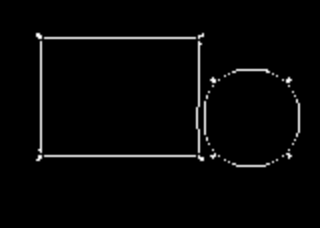
\includegraphics[width=\columnwidth]{canny_test_output.png}
\caption{Final edge map produced by the sequential Canny baseline for the
synthetic $160\times120$ input image.}
\label{fig:test-output}
\end{figure}

\section{Correctness Validation}

Correctness is evaluated at multiple levels.

First, the program must preserve the input dimensions and produce a valid
8-bit output edge map. Second, intermediate images can be written and
visually inspected after grayscale conversion, Gaussian filtering, Sobel
processing, and non-maximum suppression. Third, the final edge map can be
compared against an independently implemented reference, such as a Python
implementation, to identify algorithmic discrepancies before parallelization.

A preliminary $160\times120$ synthetic-image test produced the expected
geometric edge structure. The measured result and visual inspection are
reported in the observed test-run subsection below; this is a correctness
sanity check rather than a statistically repeated performance benchmark.

\section{Parallelization Opportunities}

The reference paper observes that pixels within a given Canny stage can be
computed independently, making the algorithm suitable for parallel
execution \cite{horvath2023}.

\begin{table}[H]
\centering
\caption{Parallelization characteristics of the logical stages.}
\begin{tabular}{p{0.27\linewidth}|p{0.62\linewidth}}
\toprule
Stage & Parallelization characteristic\\
\midrule
Grayscale &
Each output pixel depends only on its own RGB values. Very high
parallelism.\\

Gaussian &
Each output pixel depends on a fixed local $5\times5$ neighborhood.
Suitable for one-output-pixel-per-thread execution and tiling.\\

Sobel &
Each output pixel uses a fixed local $3\times3$ neighborhood. Highly
parallelizable; memory access and mathematical operations are important
performance considerations.\\

NMS &
Each output pixel examines its local neighbors along its gradient
direction. The operation is still pixel-local and highly parallelizable.\\

Threshold &
Each output pixel is classified independently. Very high parallelism.\\

Hysteresis &
Weak-edge connectivity introduces neighbor-dependent propagation, making
this stage substantially more difficult to parallelize efficiently.\\
\bottomrule
\end{tabular}
\end{table}

This decomposition provides a direct starting point for a CUDA
implementation. In particular, the grayscale, Gaussian, Sobel, and NMS
loops can be mapped to GPU threads, while Gaussian and Sobel are natural
candidates for shared-memory tiling.

The reference paper uses $16\times16$ CUDA thread blocks and shared-memory
tiling for its convolution stages \cite{horvath2023}. Its profiling also
identifies Sobel as an important bottleneck and discusses memory access and
the cost of gradient magnitude and direction calculations as optimization
targets.

\section{Conclusion}

This milestone establishes the sequential reference implementation required
before parallelization. The implementation follows the Canny pipeline used
by the primary reference and uses a straightforward single-threaded C
implementation with explicit per-stage timing.

The resulting baseline provides two essential resources for subsequent
milestones: a correctness reference and a quantitative performance
denominator. Future parallel implementations can be validated against the
same output and evaluated using speedup,

\begin{equation}
\mathrm{Speedup}
=
\frac{T_{\mathrm{seq}}}{T_{\mathrm{parallel}}}.
\end{equation}

The most promising parallel targets are the pixel-local grayscale,
convolution, Sobel, NMS, and thresholding stages. Hysteresis presents a more
challenging connectivity problem and will require additional consideration
during the parallel implementation phase.

\section*{Implementation Notes}

The supplied source file is intended to be compiled as a standalone C
program. The default threshold values are 50 and 100 but can be changed on
the command line.

\begin{lstlisting}[language=C]
clang -std=c11 -O0 -Wall -Wextra \
      -o canny_baseline canny_baseline.c -lm

./canny_baseline input.ppm output.pgm 50 100
\end{lstlisting}

For an optimized CPU baseline:

\begin{lstlisting}[language=C]
clang -std=c11 -O2 -Wall -Wextra \
      -o canny_baseline_O2 canny_baseline.c -lm
\end{lstlisting}


\section*{Appendix: Sequential C Source Code}

The complete source used for the measured run is included below. The source
implements the five-stage Canny pipeline as a single-threaded C program,
including PPM input, PGM output, per-stage timing, zero-padded convolution,
Sobel magnitude and direction, non-maximum suppression, and stack-based
8-connected hysteresis. The source file is also supplied separately with
the submission.

\lstinputlisting[language=C,basicstyle=\ttfamily\tiny,breaklines=true,frame=single,
columns=fullflexible,showstringspaces=false]{canny_baseline.c}

\begin{thebibliography}{00}

\bibitem{horvath2023}
M. Horvath Jr., M. Bowers, and S. Alawneh,
``Canny Edge Detection on GPU using CUDA,''
in \emph{2023 IEEE 13th Annual Computing and Communication Workshop and
Conference (CCWC)}, 2023, pp. 419--425,
doi: 10.1109/CCWC57344.2023.10099273.

\bibitem{cheikh2012}
T. L. Ben Cheikh, G. Beltrame, G. Nicolescu, F. Cheriet, and S. Tahar,
``Parallelization strategies of the canny edge detector for multi-core CPUs
and many-core GPUs,''
in \emph{2012 10th IEEE International NEWCAS Conference},
Montreal, QC, Canada, 2012, pp. 49--52.

\bibitem{rahamneh2019}
S. Rahamneh and L. Sawalha,
``An OpenCL-Based Acceleration for Canny Algorithm Using a Heterogeneous
CPU-FPGA Platform,''
in \emph{2019 IEEE 27th Annual International Symposium on Field-Programmable
Custom Computing Machines (FCCM)}, 2019, p. 322.

\bibitem{luo2008}
Y. Luo and R. Duraiswami,
``Canny edge detection on NVIDIA CUDA,''
in \emph{2008 IEEE Computer Society Conference on Computer Vision and
Pattern Recognition Workshops}, 2008, pp. 1--8.

\end{thebibliography}

\end{document}
